\chapter*{Proposition 25}



\begin{figure*}[ht]
    \begin{center}
    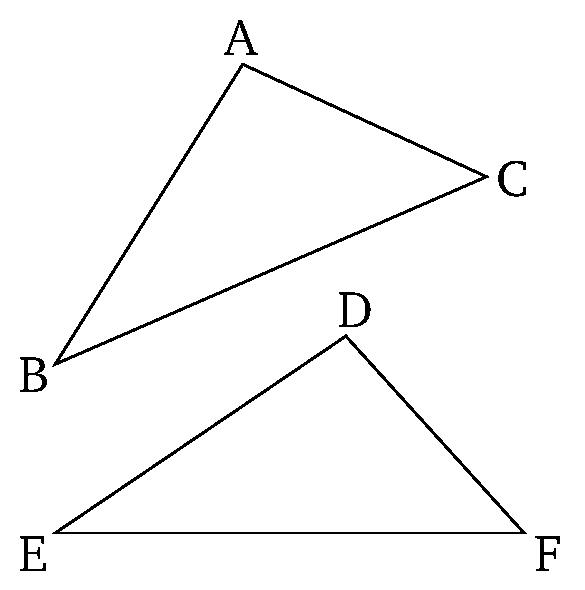
\includegraphics[width=0.5\linewidth]{figures/fig25e.eps}
    \label{fig:prop_25}
    \end{center}
\end{figure*}

If two triangles have two sides equal to two sides, respectively,
but (one) has a base greater than the base (of the other), then (the former triangle) will also have the angle encompassed by the equal straight-lines greater than the (corresponding) angle (in the latter).

Let $ABC$ and $DEF$ be  two triangles having the two sides $AB$ and $AC$
equal to the two sides $DE$ and $DF$, respectively (That is), $AB$ (equal) to $DE$, and $AC$ to $DF$. And let the base $BC$ be greater than the base $EF$. I say that angle
$BAC$ is also greater than $EDF$.

For if not, ($BAC$) is certainly either equal to, or less than, ($EDF$). In fact, $BAC$ is not equal to
$EDF$. For then the base $BC$ would also have been equal to the base $EF$ [Prop.~1.4]. But it is not.
Thus, angle $BAC$ is not equal to $EDF$. Neither, indeed, is $BAC$ less
than $EDF$. For then the base $BC$ would also have been less than the base $EF$ [Prop.~1.24].
But it is not. Thus, angle $BAC$ is not less than $EDF$. But it was  shown
that ($BAC$ is) not equal (to $EDF$) either. Thus, $BAC$ is greater than $EDF$.

Thus, if two triangles have two sides equal to two sides, respectively,
but (one) has a base greater than the base (of the other), then (the former triangle) will also have the angle encompassed by the equal straight-lines greater than the (corresponding) angle (in the latter). (Which is) the
very thing it was required to show.


\section*{Commentary}

\begin{proposition}\label{proposition_25}\lean{Elements.Book1.proposition_25}\leanok
    $\triangle~ABC$ and $\triangle~DEF$ are two triangles s.t. $|AB|=|DE|$, $|AC|=|DF|$, and $|BC|~>~|EF|$. Then, $\angle~BAC~>~\angle~EDF$.
\end{proposition}
\begin{proof}
    \uses{proposition_4,proposition_24}\leanok
    See the original proof by Euclid.
\end{proof}
